\clearpage
\section{Implementation on Quartus}
\label{sec:implementation_on_quartus}

\subsection{Warnings}
The synthesis of the project on the Altera DE2 development board generates some warnings that are safe for the project, but it is important to analyze them to ensure the correct operation of the device. \\
The analysis of the warnings is separated for each module and for the main project that connects them together.

\subsubsection{LCD module}
The LCD module generate a lot of waring due to truncation of signals. \\
The first truncation warnings are as follows.

\begin{warningbox}[Warning]
    \text{Warning (10230): Verilog HDL assignment warning at lcd\_driver.v(*):} \newline
    \text{truncated value with size 64 to match size of target (32)}
\end{warningbox}

\noindent
They are generated for the \texttt{localparam} inside the \texttt{lcd\_driver} module, which contains the values of clock cycles to wait for a specific temporal delay.

\begin{lstlisting}[language=Verilog]
    localparam [31:0] wait40us = (CLK_FREQ/1000000)*40; 
    localparam [31:0] wait1ms = (CLK_FREQ/1000)*1; 
    localparam [31:0] wait2ms = (CLK_FREQ/1000)*2; 
    localparam [31:0] wait10ms = (CLK_FREQ/1000)*10; 
    localparam [31:0] wait20ms = (CLK_FREQ/1000)*20; 
    localparam [31:0] wait100ms = (CLK_FREQ/1000)*100; 
    localparam [31:0] wait2s = CLK_FREQ*2; 
\end{lstlisting}

\noindent
The operation on the right is performed automatically at \(64 bits\). \\
The other truncation warnings refer to the initialization file for the LUT.

\begin{warningbox}[Warning]
    \text{Warning (10230): Verilog HDL assignment warning at text\_lut\_init.txt(*):} \newline \text{truncated value with size 12 to match size of target (9)}
\end{warningbox}

\noindent
The instantiated \texttt{rom} has \(9 bit\) elements but is initialized with a hexadecimal file; for this reason, the first three bits are truncated, and the memory initialization file generated contains \(9 bit\) binary elements. \\
To allow, in the future, to add other page on the LCD, some memory location of the \texttt{rom} are left uninitialized, and this generate another warning.

\begin{warningbox}[Warning]
    \text{Warning (10850): Verilog HDL warning at text\_lut.v(16):} \newline
    \text{number of words (437) in memory file does not match the number of elements in the} \newline
    \text{address range [0:2047]}
\end{warningbox}

\newpage
\noindent
The instantiated \texttt{rom} memory is a read-only memory, so all the pins needed to write the memory are fixed at zero, generating the following warnings.

\begin{warningbox}[Warning]
    \text{Warning (10030): Net "rom.data\_a" at text\_lut.v(12) has no driver or initial value, using a} \newline
    \text{default initial value '0'} \newline
    \text{Warning (10030): Net "rom.waddr\_a" at text\_lut.v(12) has no driver or initial value, using a} \newline
    \text{default initial value '0'} \newline
    \text{Warning (10030): Net "rom.we\_a" at text\_lut.v(12) has no driver or initial value, using a} \newline
    \text{default initial value '0'}
\end{warningbox}

\subsubsection{DDFS module}
The DDFS module generates only truncation warnings due to the operations that are performed by default with signed integers at \(64 bits\).

\begin{warningbox}[Warning]
    \text{Warning (10230): Verilog HDL assignment warning at ddfs.v(*):} \newline
    \text{truncated value with size 64 to match size of target (12)} \newline
    \text{Warning (10230): Verilog HDL assignment warning at ddfs.v(*):} \newline
    \text{truncated value with size 64 to match size of target (10)}
\end{warningbox}

\noindent
The last warnings of this module are referred to the \texttt{rom} instance and are the same of the LCD module.

\begin{warningbox}[Warning]
    \text{Warning (10030): Net "rom.data\_a" at sin\_lut.v(17) has no driver or initial value, using a} \newline
    \text{default initial value '0'} \newline
    \text{Warning (10030): Net "rom.waddr\_a" at sin\_lut.v(17) has no driver or initial value, using a} \newline
    \text{default initial value '0'} \newline
    \text{Warning (10030): Net "rom.we\_a" at sin\_lut.v(17) has no driver or initial value, using a} \newline
    \text{default initial value '0'}
\end{warningbox}

\subsubsection{Keypad frequency module}
This module produce only truncation warnings due to the operations that are performed by default with signed integers at \(64 bits\).

\begin{warningbox}[Warning]
    \text{Warning (10230): Verilog HDL assignment warning at keypad\_freq\_sel\_module.v(49):} \newline
    \text{truncated value with size 64 to match size of target (32)}
\end{warningbox}

\noindent
Other truncation warnings are generated from the DDFS frequency converter module

\begin{warningbox}[Warning]
    \text{Warning (10230): Verilog HDL assignment warning at DDFS\_frequency\_converter.v(*):} \newline
    \text{truncated value with size 65 to match size of target (7)}
\end{warningbox}

\newpage
\noindent
This warning come from the following part of code

\begin{lstlisting}[language=Verilog]
    fw_1000000 <= (mult_1000000*K)>>54;
    fw_100000 <= (mult_100000*K)>>54;
    fw_10000 <= (mult_10000*K)>>54;
    fw_1000 <= (mult_1000*K)>>54;
    fw_100 <= (mult_100*K)>>54;
    fw_10 <= (mult_10*K)>>54;
    fw_2 <= (mult_2*K)>>54;
\end{lstlisting}

\noindent
where \texttt{mult\_*} contains the value of the frequency multiplied by powers of \(10\). \\
The value is shifted \(54\) times to the right, which is equivalent to dividing the value by \(2^{54}\).\\
This value can be stored in \(7 bits\), but the multiplied frequency needs \(65 bits\) to be represented, for this reason Quartus report a warning.


\subsubsection{Other warnings}
The other warning are related to the connection of the GPIOs and the instance or the optimization of the logic block inside the FPGA. \\
The optimization warning are as follows

\begin{warningbox}[Warning]
    \text{Warning (14284): Synthesized away the following node(s):} \newline
    \text{\quad $\Rdsh$ Warning (14285): Synthesized away the following RAM node(s):
} \newline
    \text{\quad \quad $\Rdsh$ Warning (14320): Synthesized away node "ddfs:inst\_ddfs\_mod ... ram\_block1a0"
}
\end{warningbox}

\noindent
The meaning of the warning is that an auto generated block has been removed due to synthesis optimization. \\
The reported example refers to a RAM block instantiated inside the \texttt{ddfs} module, but there are other similar warnings referring to DSP multiplier blocks instantiated inside the \texttt{keypad\_freq\_sel\_module}. \\
The GPIOs warning instead are different, the first type of GPIO warning are like follows

\begin{warningbox}[Warning]
    \text{Warning (13024): Output pins are stuck at VCC or GND} \newline
    \text{\quad $\Rdsh$ Warning (13410): Pin "LCD\_RW" is stuck at GND} \newline
    \text{\quad $\Rdsh$ Warning (13410): Pin "LCD\_ON" is stuck at VCC} \newline
    \text{\quad $\Rdsh$ Warning (13410): Pin "LCD\_BLON" is stuck at VCC} \newline
    \text{\quad $\Rdsh$ Warning (13410): Pin "VGA\_BLANK" is stuck at VCC} \newline
    \text{\quad $\Rdsh$ Warning (13410): Pin "VGA\_SYNC" is stuck at VCC} \newline
    \text{\quad $\Rdsh$ Warning (13410): Pin "HEX7[*]" is stuck at VCC}
\end{warningbox}

\noindent
This warning is normal for this design because some output pins of the FPGA are connected to the \texttt{blank} and \texttt{synch} pins of the VGA DAC, which are not used and are always disabled. \\
Other disabled pins are the \texttt{blon}, \texttt{rw}, and \texttt{on} pins of the LCD, used to set it in write mode and to keep the backlight always on. \\
The last disabled output pins are the seven-segment pins of the last seven-segment display, which are turned off because the display is not used. \\
There are two other types of GPIOs warning, because for the design has been used a \texttt{.qsf} file to automatically configure the output pins, but some of the pin are not used in the project, for this reason Quartus report them

\begin{warningbox}[Warning]
    \text{Warning (15705): Ignored locations or region assignments to the following nodes} \newline
    \text{\quad $\Rdsh$ Warning (15706): Node " ... " is assigned to location or region, but does not exist in design}
\end{warningbox}

\newpage
\noindent
furthermore some of the output pins have no defined the output capacitance value, so the software assign the default value of \(0 pF\) to all of them

\begin{warningbox}[Warning]
    \text{Warning (306006): Found 103 output pins without output pin load capacitance assignment}
\end{warningbox}

\newpage

\subsection{Timing analyzer}
To setup the timing analyzer is important to write the \texttt{.sdc} file where are defined the clock settings and the timing constrain for the input and output pins.

\subsubsection{Timing configuration file}
The clock signals in this project are three:

\begin{itemize}
    \item \texttt{CLOCK\_50} \\
    is the \(50\ \text{MHz}\) clock from the oscillator on the DE2 board.

    \item \texttt{CLOCK\_PLL} \\
    is the clock output of the PLL. This clock source is generated from the \texttt{CLOCK\_50} clock by multiplying it by 7/5.\\
    This is a \(70\ \text{MHz}\) clock source with the same phase as \texttt{CLOCK\_50}.

    \item \texttt{CLK\_FREQ\_DIV} \\
    is the output of the frequency divider instantiated inside the \texttt{ddfs} module.\\
    The problem with this clock source is that the frequency can be selected through the external pins of the module; for the analysis, it has been configured at its maximum frequency, which is \texttt{CLOCK\_PLL} divided by two.

\end{itemize}

\noindent
the part of code used to set up the clock signals is the following

\vspace{0.5cm}
\begin{lstlisting}[language=sdc, caption=Clock settings for timing analyzer]
    create_clock 
        -name {CLOCK_50} 
        -period 20.000 
        -waveform {0.000 10.000} 
        { CLOCK_50 }
        
    create_generated_clock 
        -name {CLOCK_PLL} 
        -source {inst_pll|altpll_component|pll|inclk[0]}
        -divide_by 5 -multiply_by 7
        -duty_cycle 50.00 -phase 0.0 -offset 0.0 
        { inst_pll|altpll_component|pll|clk[0] }
        
    create_generated_clock 
        -name {CLK_FREQ_DIV} 
        -source {inst_pll|altpll_component|pll|clk[0]} 
        -divide_by 2 -multiply_by 1 
        -duty_cycle 50.00 
        { ddfs:inst_ddfs_mod|freq_divider_DDFS:f_div_inst|clk_out }
    
\end{lstlisting}
\vspace{0.5cm}

\newpage
\noindent
Now that we have defined the clock, we must add the input and output timing constrain. \\
First we define the asynchronous input and output pins, in our case the asynchronous pins are the
\begin{itemize}
    \item Switch input pins
    \item Seven segment display output pins
    \item led output pins
    \item \texttt{GPIO\_0} pins \\
    this pins are connected the row of the keypad module, the pression of a button of the keypad can be asynchronous and the input is protected with a latch chain.
\end{itemize}

the part of code used to setup the asynchronous path is the following

\vspace{0.5cm}
\begin{lstlisting}[language=sdc, caption=Setup asynchronous paths]
    set_false_path 
        -from [get_ports {GPIO_0[0] GPIO_0[1] GPIO_0[2] GPIO_0[3] SW[*]}]
    set_false_path 
        -to [get_ports {HEX0[*] HEX1[*] ... HEX5[*] HEX6[*] HEX7[*]}]
    set_false_path 
        -to [get_ports {LEDR[*] LEDG[*]}]
    
\end{lstlisting}
\vspace{0.5cm}

\noindent
Now it is time to set the timing constraints for the synchronized outputs.\\
To do this, we use the \texttt{set\_input\_delay} and \texttt{set\_output\_delay} commands.\\
These commands take two parameters: \texttt{-clock}, which is the reference clock for the specified input or output, and \texttt{-min} or \texttt{-max}, which refer to hold and setup timing constraints, respectively, and are referenced to the clock edge, as shown in \autoref{fig:min_max_delay}.

\vspace{0.5cm}
\begin{figure}[h!]
    \centering
    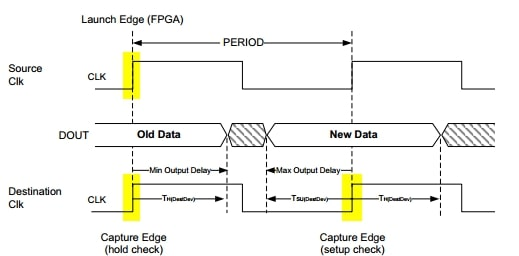
\includegraphics[width=0.6\textwidth]{img/min_max_delay.jpg}
    \caption{min and max delay timing interpretation}
    \label{fig:min_max_delay}
\end{figure}
\vspace{0.5cm}

\newpage
\noindent
For the GPIO outputs, which are connected to the keypad, and for the LCD outputs, the signals are synchronized with the \texttt{CLOCK\_PLL} source; however, the devices driven by these signals do not have a clock input. \\
For the LCD, the timing constraints are controlled by the \texttt{lcd\_driver}, and the keypad is a passive device, so it does not have digital circuits for synchronization. \\
For this reason, the constraints for these pins are arbitrary. \\
For the VGA output, we use the datasheet values for setup and hold times (respectively \(1.5ns\) and \(2.5ns\)) and choose slightly larger values to ensure safe operation.
The code to set up these timing constraints is the following

\vspace{0.5cm}
\begin{lstlisting}[language=sdc, caption=Setup synchronous paths]
    #the LCD and GPIO_1 outputs are not synchronized; 
    #therefore, the clock limits within a cycle are arbitrary
    set_output_delay 
        -min 1 [get_ports {GPIO_1[0] GPIO_1[1] GPIO_1[2] GPIO_1[3]}] 
        -clock [get_clocks CLOCK_PLL]
    set_output_delay 
        -max 1 [get_ports {GPIO_1[0] GPIO_1[1] GPIO_1[2] GPIO_1[3]}] 
        -clock [get_clocks CLOCK_PLL]
    set_output_delay 
        -min 1 [get_ports LCD*] 
        -clock [get_clocks CLOCK_PLL]
    set_output_delay 
        -max 1 [get_ports LCD*] 
        -clock [get_clocks CLOCK_PLL]
    
    #from datasheet min = thold = 2.5ns; max = tsetup = 1.5ns
    #we take some margin
    set_output_delay 
        -min 3 [get_ports VGA*] 
        -clock [get_clocks CLK_FREQ_DIV]
    set_output_delay 
        -max 2 [get_ports VGA*] 
        -clock [get_clocks CLK_FREQ_DIV]
    
\end{lstlisting}
\vspace{0.5cm}

\newpage
\subsubsection{Timing slack and critical path}
The timing analyzer uses the library of the FPGA macro-cells to verify that the timing constraints are respected for both the slow and fast models.\\
The slow model is used to check the maximum frequency of the clock sources (at a temperature of \(85^\circ C\)) and the setup timing constraints.\\
The fast model is used to verify that hold time violations do not occur (at a temperature of \(0^\circ C\)).

\paragraph{Slow model} \quad \\
As we can see in \autoref{fig:f_max}, the maximum calculated frequency for each clock source is higher than the frequency used.

\vspace{0.5cm}
\begin{figure}[h!]
    \centering
    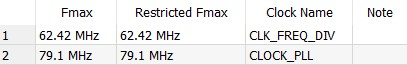
\includegraphics[width=0.6\textwidth]{img/Fmax.jpg}
    \caption{Maximum clock frequency for every clock source}
    \label{fig:f_max}
\end{figure}
\vspace{0.5cm}

\noindent
The maximum frequency is a consequence of setup time violations; in fact, from the setup time slack, we can calculate the maximum frequency for each clock source. \\
The maximum frequency is only computed for paths where the source and destination registers or ports are driven by the same clock.

\vspace{0.5cm}
\begin{figure}[h!]
    \centering
    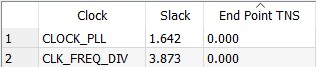
\includegraphics[width=0.45\textwidth]{img/Setup_slack.jpg}
    \caption{Setup time slack}
    \label{fig:setup_slack}
\end{figure}

\noindent
The slack reported in \autoref{fig:setup_slack} is related to the entire system, so the value represents the worst slack considering the interaction of the two clock sources. \\
The two paths that reduce the slack of the clock sources are shown in \autoref{fig:CLK_FREQ_DIV_slack} and in \autoref{fig:CLOCK_PLL_slack}

\vspace{0.5cm}
\begin{figure}[h!]
    \centering
    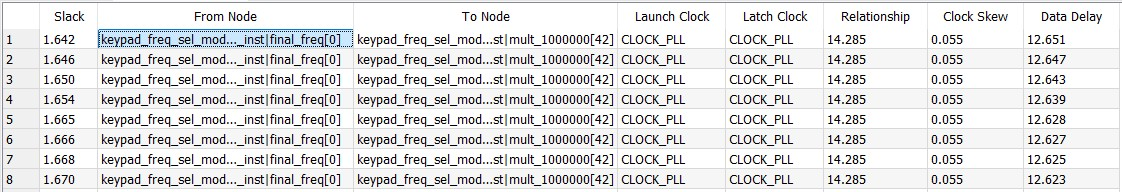
\includegraphics[width=1\textwidth]{img/CLOCK_PLL slack.jpg}
    \caption{CLOCK\_PLL setup time slack}
    \label{fig:CLOCK_PLL_slack}
\end{figure}

\begin{figure}[h!]
    \centering
    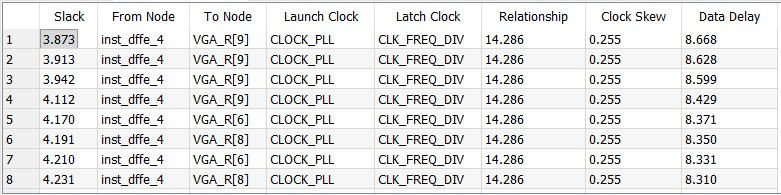
\includegraphics[width=0.8\textwidth]{img/CLK_FREQ_DIV slack.jpg}
    \caption{CLK\_FREQ\_DIV setup time slack}
    \label{fig:CLK_FREQ_DIV_slack}
\end{figure}

\newpage
\noindent
\paragraph{Critical path} \quad \\
From the analysis done with the slow model for the setup time slack,we can see that for the \\
\texttt{CLOCK\_PLL} source, the critical path is referred to the shift and add operation done into the \\
\texttt{DDFS\_frequency\_converter} module

\begin{lstlisting}[language=Verilog]
    mult_1000000 <=
    (final_freq<<19)+(final_freq<<18)+(final_freq<<17)+(final_freq<<16)
    +(final_freq<<14)+(final_freq<<9)+(final_freq<<6)
\end{lstlisting}

\noindent
For the \texttt{CLK\_FREQ\_DIV} source, indeed the critical path came from the connection between the mirror input of the \text{DDFS} module and the DAC output. \\
The critical path is referred to this two combinational blocks inside the module

\begin{lstlisting}[language=Verilog]
    if(mirror_x && mirror_y) begin
        //third quarter or fourth quarter
            ...
            
    end else if(mirror_x) begin
        //second quarter or fourth quarter
            ...
            
    end
\end{lstlisting}

\begin{lstlisting}[language=Verilog]
    if(mirror_y)
        //second quarter or fouth quarter
            ...
\end{lstlisting}

\noindent
This blocks was previously analyzed in
\autoref{sec:description_of_the_architecture} (\autoref{lst:DDFS_output_calculation} and \autoref{lst:DDFS_address}). \\
In the Chip Planner, we can see where these two critical paths are located inside the FPGA.

\begin{figure}[h!]
    \centering
    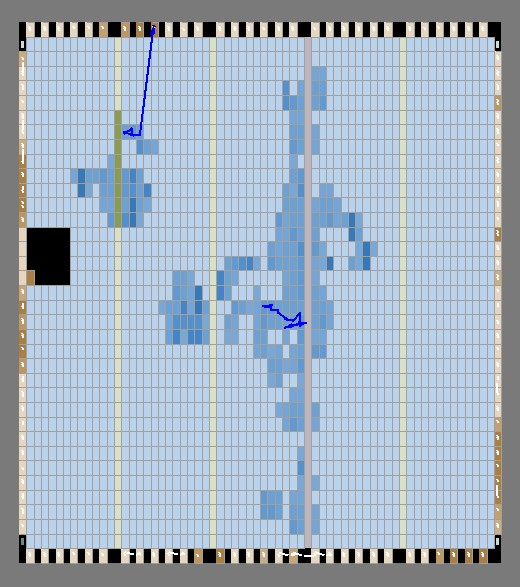
\includegraphics[width=0.5\textwidth]{img/Chip_planner_critical_path.jpg}
    \caption{Critical Path shown in the Chip Planner}
    \label{fig:Chip_planner_critical_path}
\end{figure}

\newpage
\paragraph{Fast model} \quad \\
The hold time slack for every clock source is shown in \autoref{fig:Hold_slack}

\begin{figure}[h!]
    \centering
    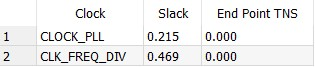
\includegraphics[width=0.5\textwidth]{img/Hold_slack.jpg}
    \caption{Hold time slack}
    \label{fig:Hold_slack}
\end{figure}

\noindent
To obtain this values of hold time slack we optimized all the path to increase the hold time slack. \\
To do this, we modified the Fitter settings as shown in \autoref{fig:fitter_settings}

\begin{figure}[h!]
    \centering
    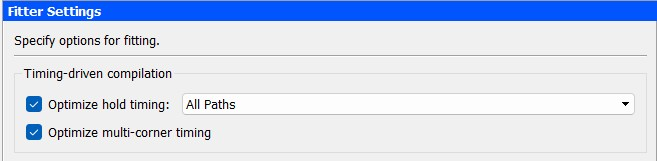
\includegraphics[width=0.8\textwidth]{img/fitter_settings.jpg}
    \caption{Fitter settings}
    \label{fig:fitter_settings}
\end{figure}

\subsection{Power consumption}
At the end of the Analysis and Synthesis, we run the Power Analyzer to check the power consumption of the project.\\
This analysis does not consider the power dissipated to drive the loads, because by default, the load capacitances are set to \(0\ \text{pF}\).\\
To perform a more accurate analysis, we have to estimate the load capacitance for each output of the circuit.

\vspace{0.5cm}
\begin{figure}[h!]
    \centering
    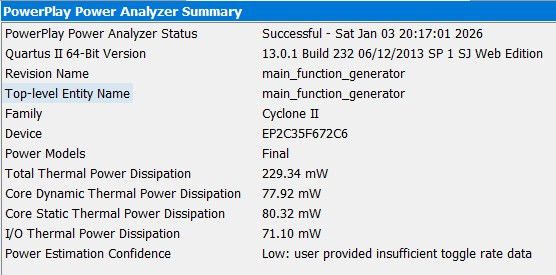
\includegraphics[width=0.6\textwidth]{img/power_analyzer_summary.jpg}
    \caption{Power analyzer summary}
    \label{fig:power_analyzer_summary}
\end{figure}

\noindent
The analyzer tool also allows you to see which parts of the power are dissipated and which portions are consumed by each block, as shown in
\autoref{fig:power_analyzer_summary_detailed}

\vspace{0.5cm}
\begin{figure}[h!]
    \centering
    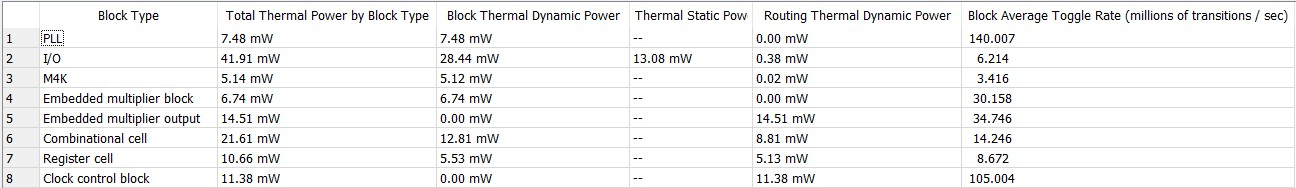
\includegraphics[width=1\textwidth]{img/power_analyzer_summary_detailed.jpg}
    \caption{Termal power dissipation by block type}
    \label{fig:power_analyzer_summary_detailed}
\end{figure}

\newpage

\subsection{Resource usage}
The internal FPGA resources used at the end of the Analysis and Synthesis operations are reported in \\ \autoref{fig:res_usage}.

\vspace{0.5cm}
\begin{figure}[h!]
    \centering
    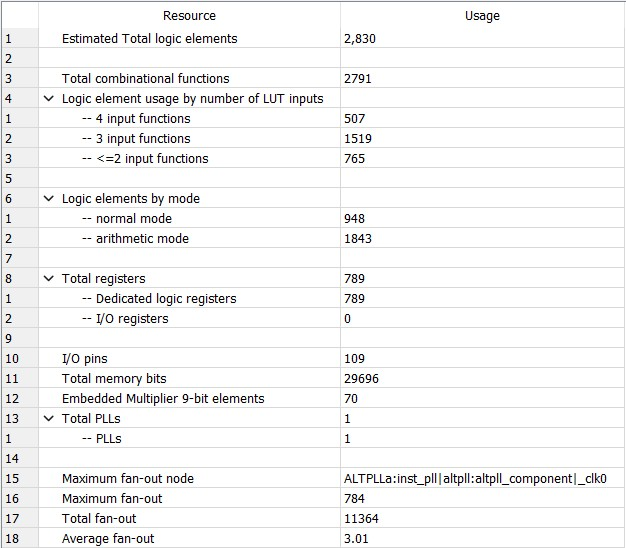
\includegraphics[width=0.8\textwidth]{img/resource usage.jpg}
    \caption{Resource usage table}
    \label{fig:res_usage}
\end{figure}
\vspace{0.5cm}

\noindent
Compared to all the resources available on the chip, the total logic elements used are only \(9\%\) of the total, and the total memory bits used are \(6\%\), as shown in \autoref{fig:flow_summary}. \\
Furthermore has been used all the embedded multiplier and one of the four internal PLL.

\vspace{0.5cm}
\begin{figure}[h!]
    \centering
    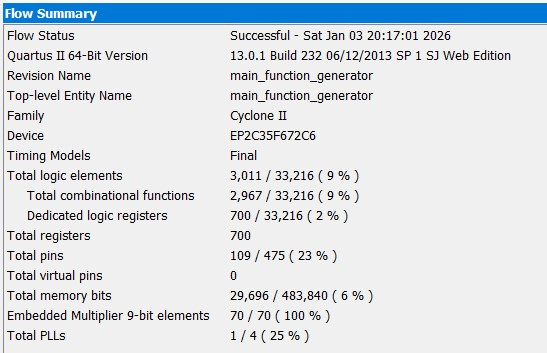
\includegraphics[width=0.8\textwidth]{img/flow_summary.jpg}
    \caption{Analysis and synthesis flow summary}
    \label{fig:flow_summary}
\end{figure}

\noindent
In the Chip Planner, we can see where are placed all the blocks of the project, inside the FPGA, as shown in \autoref{fig:chip_planner}

\vspace{0.5cm}
\begin{figure}[h!]
    \centering
    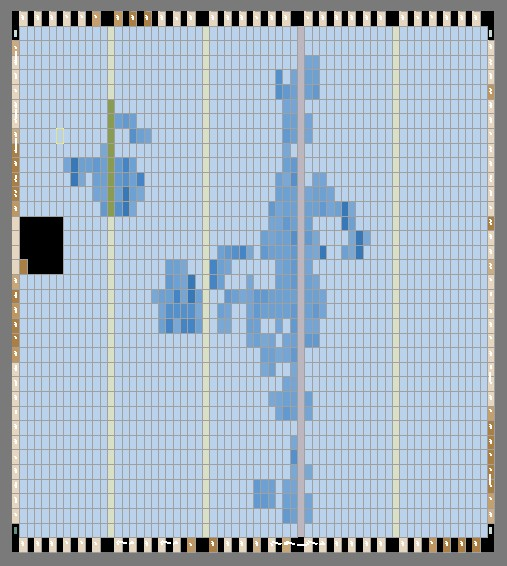
\includegraphics[width=0.8\textwidth]{img/chip_planner.jpg}
    \caption{Chip Planner}
    \label{fig:chip_planner}
\end{figure}
\vspace{0.5cm}
